\chapter{Experimental Facilities}

\section{The Relativistic Heavy Ion Collider (RHIC)}

\begin{figure}
  \begin{center}
    \includegraphics[width=0.8\textwidth]{figures/rhic-from-above}
  \end{center}
  \caption{The RHIC accelerator complex. Polarized protons are generated in
  OPPIS (not shown) and pass through the Linac, Booster, and AGS on their way
  to RHIC.}
  \label{fig:rhic}
\end{figure}

The Relativistic Heavy Ion Collider (RHIC) is an intersecting storage ring
located at Brookhaven National Laboratory in Upton, New York. Unusually
versatile for a collider, RHIC uses two independent superconducting rings to
collide beams of ions with mass numbers separately ranging from one to 197.
Recent beam configurations include protons on protons, deuterons on gold,
copper on copper, and gold on gold. Figure \ref{fig:rhic} shows a schematic
view of the RHIC accelerator complex. The main RHIC ring has a 3.8 kilometer
circumference and is comprised of six straight sections and six curved
sections. Collisions between the beams occur in the middle of each straight
section; four experimental halls are situated at the two (BRAHMS), six (STAR),
eight (PHENIX), and ten o'clock (PHOBOS) positions.

RHIC relies on a complex of smaller accelerators to prepare ion beams for
injection into the main ring. This work focuses on the systems used to
polarize and accelerate beams of protons, thus avoiding further discussion of
the Tandem Van de Graff generator used exclusively in heavy ion operations.
Polarized protons are produced using OPPIS \cite{Zelenski:2002gb,
Zelenski:2008zza}, an optically-pumped polarized ion source which typically
generates 0.5 mA, 400 $\mu$s pulses of ions, corresponding to
$\mathrm{9x10^{11}}$ ions per pulse. The pulsed nature of the beam is crucial
to achieving the RHIC design luminosity of
$\mathrm{2x10^{32}~cm^{-2}~s^{-1}}$. OPPIS polarizes protons by passing them
through a rubidium vapor pumped with circularly polarized laser light in a
strong magnetic field. The $\mathrm{H^+}$ ions pick up a polarized rubidium
electron through collisions in the vapor, and magnetic fields cause the
electron polarization to be transferred to the nucleus. Finally, the hydrogen
atoms are ionized to $\mathrm{H^-}$ when they pass through a sodium vapor.

The pulses of 35 keV $\mathrm{H^-}$ ions produced by OPPIS are accelerated by
the LINAC, Booster, and AGS on their way to RHIC. The LINAC strips off the
electrons and accelerates the protons to a kinetic energy of 200 MeV with an
efficiency of approximately 50\%. It injects the remaining $\sim
\mathrm{4x10^{11}}$ ions into the Booster ring in a single bunch. The Booster
accelerates the protons to 1.5 GeV and passes them on to the Alternating
Gradient Synchrotron (AGS), which accelerates them to the RHIC injection
energy of 25 GeV. RHIC propels the $\sim \mathrm{2x10^{11}}$ protons remaining
in each bunch to the desired collision energy, which can range from 30 GeV to
250 GeV. This work analyzes data collected with a beam energy of 100 GeV. More
details of the RHIC accelerator complex are available in references
\cite{Harrison:2003sb, Hahn:2003sc, Alekseev:2003sk}.

\subsection{Spin Dynamics and Siberian Snakes}

The evolution of the spin direction of a beam of polarized protons in external
magnetic fields is governed by the Thomas-BMT equation \cite{Thomas:1927yu,
Bargmann:1959gz},
%
\begin{equation}
  \frac{d\vec{P}}{dt} = -\left(\frac{e}{\gamma m}\right)[(G\gamma + 1) \vec{B}_{\perp} + (G + 1) \vec{B}_{\parallel}] \times \vec{P}.
\end{equation}
%
Comparing this equation with the Lorentz force equation governing the orbital
motion,
%
\begin{equation}
  \frac{d\vec{v}}{dt} = -\left(\frac{e}{\gamma m}\right)[\vec{B}_{\perp}] \times \vec{v},
\end{equation}
%
one realizes that, in a pure vertical magnetic field, the spin rotates
G$\gamma$ + 1 times faster than the orbital motion. This factor, referred to
as the spin tune $\nu_{sp}$, gives the number of full spin precessions for
every orbit.

An accelerating beam in a storage ring encounters depolarizing resonances
whenever the spin tune is equal to an integer multiple of the frequency with
which a spin-depolarizing magnetic field is encountered. In the simplest case,
a depolarizing field can be introduced by a magnet error or misalignment. For
these \textit{imperfection resonances}, the resonance condition is just
$G\gamma = n$. If $G\gamma$ is non-integral, the beam sees the depolarizing
field at a different point in its precession on each revolution, and the
effects tend to cancel out. The focusing fields themselves can also be a
source of depolarization; for these \textit{intrinsic resonances} the
resonance condition is $G\gamma = kP \pm \nu_y$, where $k$ is an integer,
$\nu_y$ is the vertical betatron tune, and $P$ is the superperiodicity.

The stable spin direction in an accelerating beam normally coincides with the
vertical magnetic field (longitudinal polarization at the interaction points
being achieved through the use of spin rotator magnets), but near a resonance
it is perturbed away from the vertical by the resonance driving fields. The
polarization loss when a beam is accelerated through one of these resonances
can be calculated analytically \cite{Froissart:1960zz}:
%
\begin{equation}
  \frac{P_f}{P_i} = 2 e^{-\pi |\epsilon|^2 / 2\alpha} -1.
\end{equation}
%
Here $\epsilon$ is the resonance strength and $\alpha$ is the change of the
spin tune per radian of the orbit angle. When the beam is slowly accelerated
($\alpha \ll |\epsilon|^2$) the stable spin direction changes adiabatically
and the result is a spin flip. In contrast, techniques such as a betatron tune
jump effectively result in $|\epsilon|^2 \ll \alpha$ and thus preserve the
polarization through the resonance. At high energies, the number and strength
of the resonances encountered make these traditional techniques impractical.
Instead, the RHIC rings employ ``Siberian Snake'' magnets
\cite{Derbenev:1978hv} which generate a 180\degree spin rotation about a
horizontal axis when the beam passes through them. In effect, the Siberian
Snakes ensure that the spin tune is an energy-independent half-integer, thus
avoiding all imperfection resonances as well as intrinsic resonances with an
appropriate choice of the betatron tune. RHIC is designed to achieve 70\%
polarization; the datasets analyzed in this work were taken with 45\% - 55\%
polarized beams, as certain elements of the accelerator complex (notably, a
Siberian Snake in the AGS) were still being commissioned.

\subsection{Polarimetry Systems\label{sec:polarimeters}}

RHIC polarimetry relies on the observation of small angle elastic scattering
in the Coulomb-Nuclear Interference (CNI) region. Two complementary varieties
of target are used: a thin carbon ribbon \cite{Jinnouchi:2004up} and a
hydrogen gas jet (H-Jet) \cite{Zelenski:2005mz, Okada:2006dd}. The carbon
ribbon boasts a large scattering cross section which allows a statistically
precise measurement of the beam polarization in a few seconds, but the
theoretical prediction for the analyzing power of this measurement includes an
unknown contribution from a hadronic spin flip amplitude. In contrast, the
hydrogen gas jet has a well-understood analyzing power but a much smaller
scattering cross section. The natural solution, then, is to calibrate the
results of the p+C CNI polarimeters with a measurement from the H-jet
polarimeter.

The p+C polarization measurements are performed using individual carbon ribbon
targets in each beam that are a mere 150 $\mathrm{\mathring{A}}$ thick.
Scatterings occur at a momentum transfer of 0.002 - 0.010 $\mathrm{GeV}^2$,
resulting in a small forward scattering angle for the proton and a recoil
carbon nucleus with less than 1 MeV of kinetic energy. Detection of the
scattered proton is not possible without drastic changes to the beam profile
at the polarimeter location, but the thinness of the target allows the recoil
nucleus to escape the target and reach one of a set of silicon strip detectors
arranged around it. The use of a thin target also allows the measurement to be
performed multiple times over the course of a beam store with acceptable
losses in luminosity.

The theoretical uncertainty in the analyzing power of the p+C measurements is
estimated to be less than 10\% \cite{Alekseev:2003sk}, but this uncertainty
can be mitigated by calibrating the results from the p+C polarimeter against
measurements performed using the hydrogen gas jet target. The use of identical
beam and target particles allows the polarization of the beam to be directly
expressed in terms of the target polarization,
%
\begin{equation}
  P_{beam} = -P_{target}\frac{\epsilon_{beam}}{\epsilon_{target}},
\end{equation}
%
and since the target polarization is precisely measured using a Breit-Rabi
polarimeter, this approach eliminates the uncertainties from the
non-perturbative hadronic spin flip amplitude. A single H-Jet polarimeter
measures the polarization in both beams. The polarimeter requires an
integration time of twenty hours to achieve a 2\% statistical uncertainty for
a single beam, but because the scattering cross section is so small this
measurement can occur concurrently with experimental data taking.

\subsection{Cogging and Bunch Patterns}

The RHIC beams are configured into 120 RF buckets capable of storing bunches
injected from the AGS. In practice, not all of these 120 buckets are filled; a
small number must be left empty as an ``abort gap'' to allow a controlled
dumping of the beam when the luminosity has dropped below a useful level for
physics data-taking. The two beams are cogged so that bunches from each beam
can pass through one another at the RHIC interaction points. During a given
RHIC store a given bunch from the ``Yellow'' beam always collides with the
same bunch from the ``Blue'' beam. The polarization of each bunch is
independently controlled at injection time, and the mapping of polarization
states to bunch numbers can vary from fill to fill, enabling a powerful
control on spin-dependent systematic uncertainties at the experiments.

\section{The Solenoidal Tracker at RHIC (STAR)}

STAR \cite{Ackermann:2002ad} is a general-purpose collider detector with
several subsystems capable of investigating a wide range of phenomena from
multiple collision types. A schematic of the detector is shown in Figure
\ref{fig:star-schematic}. STAR acquires data in \textit{runs}, typically of 30
to 45 minutes duration, in which several hundred thousand events will be
recorded. If a problem is discovered with a run during acquisition,
reconstruction, or analysis, that run can be cleanly discarded without the
loss of a large number of good events. Five STAR subsystems are of interest in
this work: the Beam-Beam Counters (BBCs), Zero Degree Calorimeters (ZDCs),
Barrel Electromagnetic Calorimeter (BEMC), Endcap Electromagnetic Calorimeter
(EEMC), and STAR's flagship subsystem, the Time Projection Chamber (TPC). The
BBCs and BEMC identify interesting events online and trigger the detector to
read them out, while the BEMC, EEMC and TPC are used to reconstruct the final
state of the event offline. The BBCs and ZDCs also allow a bunch
crossing-dependent measure of the beam luminosities, which is essential to
normalize spin-dependent asymmetries. These and other subsystems are described
in greater detail in \cite{RHIC-Special-Issue}.

\begin{figure}
  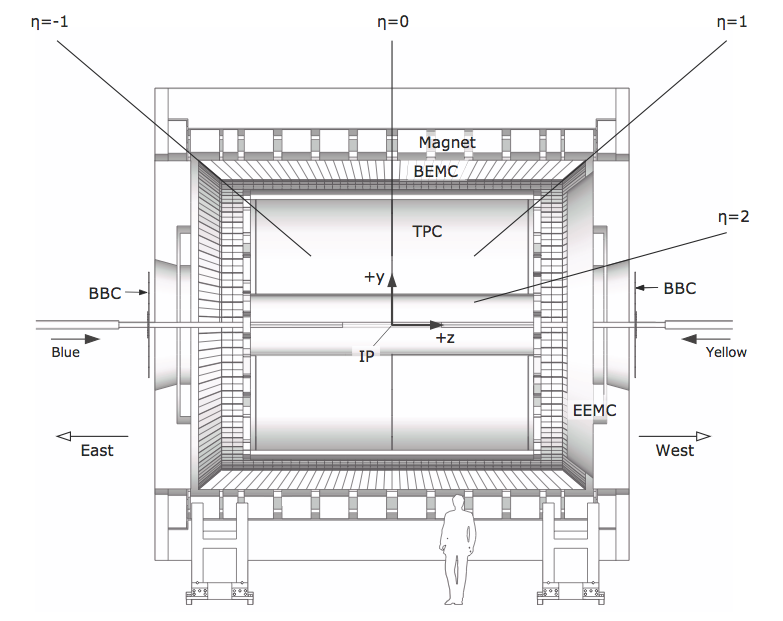
\includegraphics[width=1.0\textwidth]{figures/star-schematic-new}
  \caption{Schematic overview of the STAR detector, identifying many of the
  detector subsystems and defining the STAR coordinate system.}
  \label{fig:star-schematic}
\end{figure}

\subsection{Trigger System}

STAR has a 3 level hardware trigger system (L0, L2, L3) \cite{Bieser:2002ah,
Adler:2002ab} allowing for the selection of rare events from the large pool of
minimum bias (MB) interactions. While the TPC and other tracking detectors
have long readout times compared to the interaction rate, the BBCs and the
BEMC are fast detectors that sample each bunch crossing at the STAR IR, and
can thus be used for efficient selection of high $p_T$ events. A typical
trigger mix consists of $\sim$10-20 separate triggers running in parallel.
Significant improvements to the STAR data acquisition system (DAQ) beyond
design specifications have increased the rate of event recording to typical
values of 30-50 Hz, with a dead-time fraction of $\sim$50\%.

The L0 trigger operates on coarse-granularity data from fast detectors and
builds a decision tree capable of completing its analysis in time with the 119
nanosecond RHIC bunch crossing interval. If the L0 trigger issues an accept
the full trigger detector data is sent to L2 for further analysis. In contrast
to L0, the L2 trigger runs on commodity hardware and its algorithms can be
written in C. It applies preliminary calibrations and can do some primitive
jet finding in the course of making its decision, but must issue that decision
in no more than 5 milliseconds. If the L2 trigger issues an accept, the slow
detectors are read out and the full event is recorded to tape. The L3 trigger
\cite{Adler:2002ab} enables online TPC track finding using a farm of commodity
servers. It was at one time a necessary component of the trigger system, but
upgrades to the data acquisition system have increased the throughput from
STAR to the RHIC Computing Facility (RCF) to the point where the $\sim$50 Hz
of events selected by the L0 and L2 trigger algorithms can be recorded to
tape. The L3 tracking output continues to serve as a useful qualitative
monitoring tool in the STAR control room.

\subsection{Beam Beam Counters\label{sec:bbc}}

The BBCs \cite{Kiryluk:2003aw} consist of two hexagonal scintillator arrays,
one immediately outside each magnet poletip 3.7~m from the interaction point.
Each array is tiled from 36 individual hexagonal scintillators read out by
wave length shifting fiber and a photomultiplier tube. The beam pipe passes
through the center of the array. The region 9.6~cm to 48~cm from the beam axis
($3.3 < |\eta| < 5.0$) is covered by 18 small hexagonal tiles. The remaining
region out to 193~cm from the beam pipe ($2.1 < |\eta| < 3.3$) is covered by
18 large hexagonal tiles. Only the small tiles are used in this analysis.
Thresholds are set well below the signal deposited by a single ionizing
particle in a tile, and a bunch crossing is recorded as having a hit based on
the relative timing between the first signal from any of the small tiles on
one side with the first signal from any of the small tiles on the other. The
timing resolution is $\sim$1~ns, sufficient to separate beam backgrounds which
should hit the two counters in succession vs. particles from a collision which
should result in both counters being struck simultaneously. A timing cut 8~ns
wide selects only coincidences with collision timing, and individual scalers
are kept for each timing bin in addition to the total in the timing gate, thus
allowing for more selective cuts offline.

In addition to defining the MB trigger condition, coincident signals in the
BBCs also serve as a luminosity monitor. In particular, tracking the number of
BBCs hits per bunch crossing allows one to measure the luminosities for each
combination of the spin states of the two beams. The ratios of these
luminosities are a crucial element in the extraction of single- and
double-spin physics asymmetries at RHIC. The absolute luminosity seen by the
BBCs is calibrated by measuring the size of the beams and the number of
colliding protons. The coincident cross section was found to be 26.1 $\pm$
1.8(stat) $\pm$ 1.8(syst)~mb, representing $87\pm8\%$ of the non-singly
diffractive pp cross section \cite{Adams:2003kv}. This translates into a
typical BBC coincidence rate for 2005(2006) data of $\sim$180(??)~kHz.

\subsection{Zero Degree Calorimeters\label{sec:zdc}}

The ZDCs \cite{Adler:2003sp} are hadron calorimeters placed 18~m upstream on
each side of the the STAR interaction point. This places them on a line with
the colliding beams but outside the final bending magnets between the two beam
lines. They are 6 hadronic interaction lengths in depth but only 10~cm wide
extending $\pm$2.7~mrad from the beam. As with the BBCs, a hit is recorded
based on a coincidence between the two ZDCs with timing consistent with
particles arriving simultaneously from the interaction point. These devices
are designed to be sensitive to neutrons from heavy ion reactions and thus are
not used as trigger detectors in the pp program. They do serve as a secondary
luminosity monitor useful for many systematic error checks. They typically
count a factor of 100 less than the BBC.

\subsection{Scaler System\label{sec:scalers}}

Signals from the L0 Trigger and the BBCs and ZDCs are processed by a set of 12
Scaler Boards \cite{scalers}. A Board is a custom VME histogramming module with
24 input bits, the combination of which maps to one of \(2^{24}\) 40 bit memory
locations on the module. 7 input bits are reserved for an encoding of the bunch
crossing number, leaving 17 for detector-specific logic. The memory location
addressed by a particular 24 bit input pattern is incremented when an event
satisfies that bit pattern. The scaler system typically tracks hits in the East
and West halves of the luminosity monitors separately, as well as a variety of
coincidences with different \(\Delta T\) requirements. Some of the boards are in
continuous operation during a STAR run, while others sample at discrete
intervals.

\subsection{Electromagnetic Calorimeters}

Electromagnetic calorimetry is an essential element of the trigger system at
STAR and is also important for many final state analyses (especially, for the
purposes of this thesis, jet reconstruction). We will focus on two calorimeter
subsystems: the BEMC \cite{Beddo:2002zx}, covering $|\eta| < 1.0$, and the
EEMC \cite{Allgower:2002zy}, which is installed only on the West side of STAR
and spans $1.09 < \eta < 2.0$. Both the BEMC and EEMC are segmented sampling
calorimeters with lead absorber layers and active plastic scintillator layers.
The BEMC is divided into 4800 projective towers spanning $\Delta \eta \times
\Delta \phi = 0.05 \times 0.05$, while the EEMC's 720 projective towers each
span 0.1 in azimuth and range in pseudorapidity coverage from $\Delta \eta =
0.057$ at $\eta = 1.09$ to $\Delta \eta = 0.099$ at $\eta = 2.0$. Both
calorimeters have a depth of at least twenty radiation lengths.

At Level 0, the BEMC and EEMC implement trigger conditions based on thresholds
in single high towers, 4x4 (4x2) trigger patches, and 20x20 (12x10) jet
patches. At Level 2 the calorimeters drive a wide variety of trigger
algorithms ranging from dijet reconstructions that span seamlessly across the
two calorimeters to heavy flavor searches doing online calculations of tower
pair invariant masses. The primary calorimeter trigger condition used in this
work is the BEMC jet patch (JP) trigger, which requires an energy sum above
threshold in one of twelve fixed collections of 400 towers each spanning
$\Delta \eta \times \Delta \phi = 1.0 \times 1.0$. In this case the Level 2
trigger algorithm is a simple accept, and the EEMC is used only for final
state jet reconstruction.

%% This table is probably not a good idea anyway.
% \begin{table}
%   \begin{center}
%     \begin{tabular}{c|cc}
%       & BEMC & EEMC\\
%       \hline
%       depth & $\geq 20~\chi_0$ & $\geq 20~\chi_0$
%     \end{tabular}
%   \end{center}
%   \caption{PID Selection Windows}
%   \label{tbl:pid-selection-windows}
% \end{table}

\subsection{Time Projection Chamber}

The TPC \cite{Anderson:2003ur} is the primary detector subsystem at STAR,
providing full azimuthal tracking of charged particles with transverse
momentum above $\sim 100$ MeV/c and $|\eta| < 1.8$, and particle
identification through measurements of ionization energy loss. It is a 4.2
meter long volume of gas bounded by an inner field cage at a radius of 50
centimeters and an outer field cage at 200 centimeters. The end caps of the
detector are held at ground potential and the central cathode membrane at
-28kV; metal rings connected by precision resistors in the field cages ensure
a uniform electric field of $\approx 135$ V/cm. The TPC sits inside a solenoid
with a field strength of 0.5 Tesla.

Charged particles ionize the P10 gas as they traverse the volume of the TPC,
producing secondary electrons that drift to the nearest end cap of the
detector. The $z$ coordinate of each point along the track is calculated by
measuring the time required for the electrons to reach the end cap and
dividing by the drift velocity. The drift velocity varies with electric field
strength and with the temperature, pressure, and composition of the gas, so
measurements of it are performed every few hours using the TPC laser system
\cite{Abele:2003aa}. Radial laser beams at known positions along the length of
the TPC ionize trace organic substances in the P10 gas; the time difference
between the arrival of electrons liberated by lasers at two different
positions allows a calculation of the drift velocity.

% could say a little more about how electron drift time is measured ... e.g. time buckets for readout pads
Each end cap is divided into twelve sectors, positioned as the hours on a
clock face, and each sector contains 45 rows of cathode pads (5,692 pads per
sector). The cathode pads are mounted on anode wires; the secondary electrons
avalanche near the anode wires, and the positive ions produced in this
avalanche generate a temporary image charge on several nearby pads. The image
charge is measured, and an analysis of the charge sharing between the pads
allows the original track $x$ and $y$ coordinates along the wire to be
reconstructed to within a small fraction of a pad width. Finally, the charge
deposited on each pad is used to calculate the particle's energy loss per unit
length due to ionization, or dE/dx.

\begin{figure}
  \includegraphics[width=1.0\textwidth]{figures/tpc}
  \caption{The STAR Time Projection Chamber (TPC). The end-caps are divided
  into twelve sectors, each with an inner and outer sub-sector. The TPC is
  divided into two by a central cathode membrane spanning the gas volume
  between the inner and outer field cages.}
  \label{fig:tpc}
\end{figure}

\subsection{Computing Facilities}

The aggregate raw data produced by all detector subsystems in STAR is on the
order of 100 MB per event. The STAR Data Acquisition System (DAQ)
\cite{Landgraf:2002zw} reduces the event size through hardware-based zero
suppression, resulting in a 10x savings for the highest multiplicity heavy ion
collisions and substantially greater savings (100x or more) for the
proton-proton collisions analyzed in this work. It then organizes the data
into DAQ files and transfers these files to tape in the RHIC Computing
Facility's HPSS hierarchical storage system, which provides 8 PB of storage
and a throughput of over 300 MB per second to the RHIC and USATLAS
experiments.

Event reconstruction and data analysis takes place on a Linux compute farm
with over 3300 cores and 1.7 PB of local storage. The STAR reconstruction
software is written in C++ and runs on Scientific Linux, a version of Red Hat
Enterprise Linux maintained by the particle physics community. The event
reconstruction code loads DAQ files from HPSS into local storage, performs
tracking and applies a variety of detector calibrations, and generates ``micro
Data Storage Tapes'' or ``$\mu$DSTs'', which contain higher-level physics
objects such as particle tracks, event vertices, and calorimeter clusters.
$\mu$DSTs are implemented using ROOT \cite{Brun:1997pa} TTrees, allowing
efficient ad-hoc and batch data analysis. The analysis presented here was
performed on a set of TTrees generated from $\mu$DSTs using a mix of custom
C++ libraries and Python scripts interfacing with the ROOT data analysis
framework.
